\documentclass[conference]{IEEEtran}
\IEEEoverridecommandlockouts
% The preceding line is only needed to identify funding in the first footnote. If that is unneeded, please comment it out.
\usepackage{cite}
\usepackage{amsmath,amssymb,amsfonts}
%\usepackage{algorithmic}
%\usepackage{graphicx}
\usepackage{textcomp}
\def\BibTeX{{\rm B\kern-.05em{\sc i\kern-.025em b}\kern-.08em
    T\kern-.1667em\lower.7ex\hbox{E}\kern-.125emX}}

\usepackage{verbatim}
\usepackage{graphicx}
\usepackage{subfigure}
\usepackage{algorithmic}
\usepackage[ruled]{algorithm}
\usepackage{color}
%\usepackage{amssymb}
%\usepackage{amsmath}
\usepackage{url}
\usepackage{wrapfig}
\usepackage{amsthm}
\usepackage{multirow}

\usepackage[papersize={8.5in,11in}, left=0.64in, right=0.64in, top=0.75in, bottom=1in]{geometry}

\newtheorem{theorem}{Theorem}
\newtheorem{lemma}{Lemma}
\theoremstyle{definition}
\newtheorem{definition}{Definition}



\begin{document}

\title{Autonomous Refueling Strategies using Vehicle-to-Infrastructure Communication in Smart Cities }

\author{
% Your names and contact info \\
%Xiao Chen \\
%Department of Computer Science, Texas State University, San Marcos, TX $78666$ \\
%Email: xc10@txstate.edu
}
\maketitle

% ------------------------------------------------------------------------------------------------- Abstract
\begin{abstract}

\end{abstract}

\begin{IEEEkeywords} feedback, forwarding, maximum transmission unit, opportunistic mobile social networks  \end{IEEEkeywords}


% ------------------------------------------------------------------------------------------------- Introduction
\vspace{-0.3cm}
\section{Introduction}
{\color{red} You write this part the last after you finish the rest of the sections.}

Intelligent Transportation Systems (ITS) \cite{Alam2016} is one of the major structures in building a safe, secure, and efficient smart city \cite{Bowerman2000}. It has noticed particular development in recent years thanks to the emergence of vehicular networks as a result of advancements in intelligent systems, wireless technologies, ad-hoc networking, and the automobile industry. Vehicular networks are formed among moving vehicles, road side units (RSUs), and pedestrians that carry communication devices. They can be deployed in rural, urban, and highway environments.  There are three main scenarios for vehicular communication: vehicle-to-vehicle (V2V), vehicle-to-infrastructure (V2I), and vehicle-to-pedestrian (V2P) \cite{Tseng2015}. Among these, V2I technologies capture vehicle-generated traffic data, wirelessly providing information such as advisories from the infrastructure to the vehicle that inform the driver of safety, mobility, or environment related conditions. State and local agencies are likely to install V2I infrastructure alongside or integrated with existing ITS equipment.

Recently, self-driving vehicles have attracted tremendous attention from all walks of life. The IEEE researchers predict that self-driving vehicles will comprise $75\%$ of total traffic on the road by the year $2040$ \cite{IEEEPrediction}.  Self-driving vehicles will provide tremendous benefits to society in terms of convenience and quality of life. Such vehicles will provide unprecedented access to transportation to those who need it most and those with limited access to public transportation. They will make road safer by reducing human errors and allow the driver to do something more productive. These benefits will not be realized unless vehicles are truly autonomous. At this technology level, the driver hands over control to the vehicle and the driver is no longer responsible for monitoring the system.  This will mean that the vehicle will be able to handle all situations that may occur on the road.

The emergence of self-driving vehicles and their networks will impose new requirements in the fields of safety messaging, traffic monitoring, lane changing, and intersection management for applications and services. Over the past few decades, researchers have extensively investigated the potential of designing communication protocols  that involve V2V \cite{Abbasi2018, Demba2018}, V2I \cite{Noh2015, Silva2018}, and V2P \cite{Bian2018, Corchero2018}.

\begin{figure}
\centering
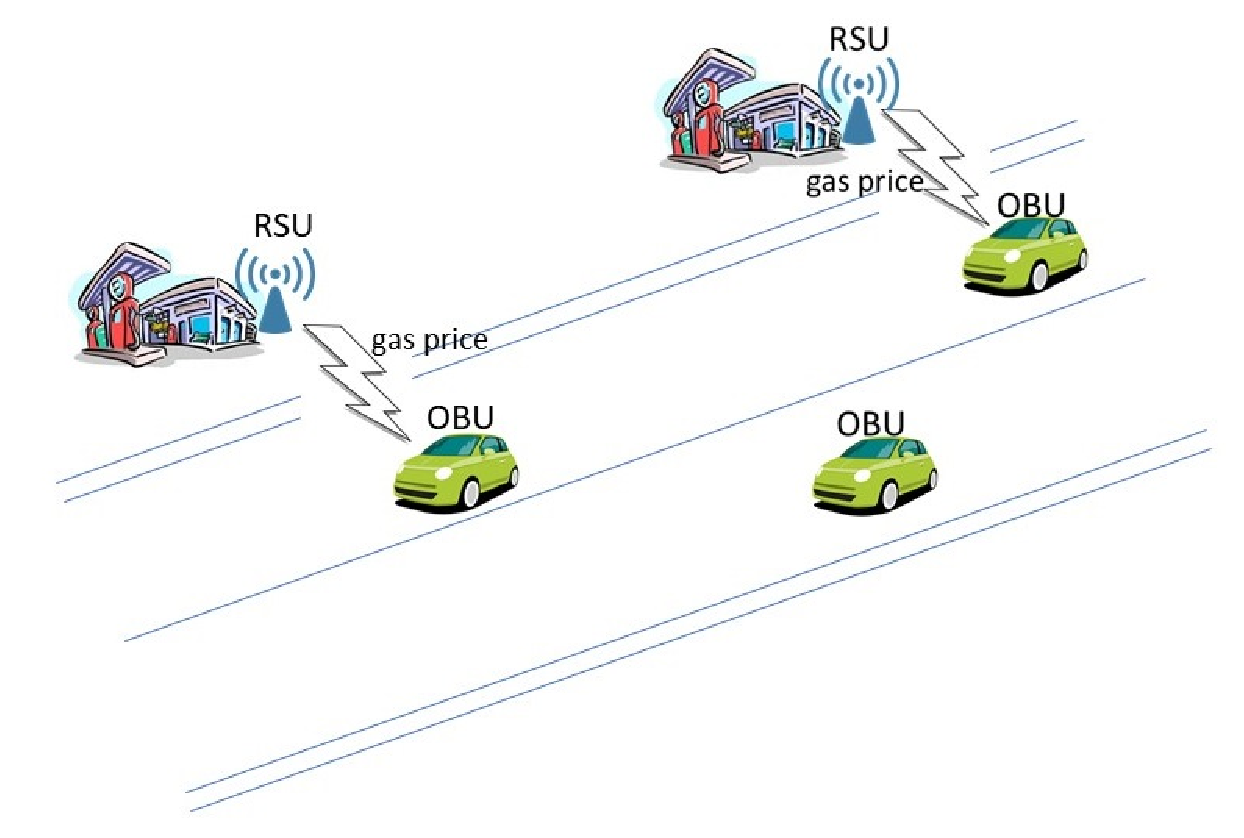
\includegraphics[width=3.08in]{v2i.eps}
\caption{RSUs at gas stations sending gas prices to OBUs in vehicles }
\label{v2i}
\vspace{-0.3cm}
\end{figure}

Several solutions to the intelligent transport systems have been installed in the vehicles and currently available on the market, such as autonomous driving \cite{Arena2018}, assisted parking systems \cite{Liu2018}, anti-collision sensors \cite{Sanjana2017}, driver notification systems \cite{Tijerina2016}, and intelligent navigation systems \cite{Zhang2016}.

In this paper, we will work on an application using V2I that, to our best knowledge, has not been discussed so far. This application is the vehicle gas adding strategy (GAS) problem. Since the self-driving vehicle has the whole control of the vehicle, it needs to decide when to stop to add gas. When a vehicle is driving on the road, it can encounter many gas stations. If its gas tank is running low, it needs to stop to add gas. We assume that gas stations can have different gas prices that can be ranked from the highest to the lowest with no ties. At each gas station, an RSU is deployed. And in each vehicle, an On Borad Unit (OBU) is installed. In V2I, RSU and OBU are the communicating nodes.  They are dedicated short-range communication (DSRC) devices. DSRC works in $5.9$ GHz band with bandwidth of $75$ MHz and approximate range of $300$ m \cite{DSRC}.   When a vehicle passes by a gas station, the RSU at the gas station  transmits the gas price of the station to the vehicle (see Figure \ref{v2i}). The goal of the vehicle is to add gas at the lowest possible price without running out of gas. We assume that once a vehicle passes a gas station, it cannot come back because an efficient self-driving vehicle wants to get to the destination as soon as possible.  We assume that a vehicle expects to compare $k$ gas stations before it makes a decision to stop. For each gas station $j$, the vehicle can only ascertain the relative rank of the gas station relative to the previous $j-1$ viewed gas stations. Under this condition, if the vehicle stops too early, it does not have the risk of running out of gas but there may be lower prices ahead. On the other hand, if the vehicle stops too late, it may not find a gas station anymore before running out of gas. So our task is find the best solution to the GAS problem. In other words, what is the best stopping rule for the vehicle to stop to add gas.

The GAS problem resembles the classic secretary problem (CSP) \cite{CSP}, where a decision maker (DM) wants to hire the best secretary out of $n$ rankable applicants for a position. But the GAS problem is different in that the number of gas stations ahead before the vehicle runs out of gas is not known while the number of applicants in CSP is fixed and known. So for the GAS problem, the focus is not the stopping rule but the starting rule. That is,  when the vehicle should start to look for a gas station so that it has the highest chance to encounter $k$ gas stations  before it runs out of gas. We propose a solution to the GAS problem which we refer to as {\em SGAS}. Our solution SGAS has two parts: the first part is to determine the starting point for the vehicle to look for a gas station so that it has the highest probability to see $k$ gas stations ahead before it runs out of gas; the second part is that once the vehicle starts looking, it will use the optimal stopping rule of CSP to stop at the gas station that most likely offers the lowest gas price. To find the best starting rule is our main task in this paper. In search of the starting rule, an intuition is that it is related to the distribution of the gas stations on the road because the more the gas stations, the later the vehicle can start looking. Reverse, otherwise. Therefore, we discuss a possible distribution of gas stations in real life:  the Poisson distribution. Then we put forward the starting rule for each distribution.  We evaluate the effectiveness of our strategies using simulations. The simulation results show that ...

The differences of our work from others and the key contributions of our work are as follows:
\begin{itemize}
\item We are the first to discuss gas adding strategy (GAS) problem of self-driving vehicles to the best of our knowledge.
\item We provide solutions to the GAS problem by discussing the Poisson distribution.
\item We demonstrate the effectiveness of our schemes analytically and experimentally by simulations.
\end{itemize}

The rest of the paper is organized as follows: Section \ref{related} references the related works;  Section \ref{problem} defines the problem;  Section \ref{solution} presents our solution;  Section \ref{analysis} gives mathematical analyzes of our solution;  Section \ref{simulations} shows the simulations; and Section \ref{conclusion} is the conclusion.



\section{Related Works} \label{related}
\subsection{Classic Secretary Problem}
In the classic secretary problem (CSP) \cite{CSP}, a DM wants to hire the best secretary out of $n$ rankable applicants for a position. The applicants are interviewed one by one in a random order.  When the DM interviews the $j$th applicant in the sequence, she gains information sufficient to rank the applicant among all applicants interviewed so far, but is unaware of the quality of yet unseen applicants.   Her objective is to find an optimal strategy or the stopping rule to maximize the probability of selecting the best applicant. The CSP can be formally stated below:

\begin{enumerate}
\item  There is a fixed and known number $n$ of applicants who can be ranked from the best $1$ to the worst $n$ without a tie competing for a single position.
\item The applicants are interviewed sequentially in a random order (with a total of $n!$ orderings with equal probability).
\item For each applicant $j$, the DM can only know the relative rank of the applicant, that is, how good the applicant is relative to the previous $j-1$ applicants.
\item Once rejected, an applicant cannot be called back later. If no candidate has been selected before the last one, the last one must be accepted.
\item The DM earns a payoff of $1$ for selecting the applicant with absolute rank $1$ in the $n$ applicants and $0$, otherwise.
\end{enumerate}


The problem has an elegant solution and the optimal (expected payoff maximizing) search policy is to interview and reject the first $t^{*}-1$ applicants and then to accept the first one thereafter with a relative rank of $1$ \cite{Gilbert1966}. The optimal cutoff can be obtained by

$t^{*} = \min \{t \geq 1: \sum_{k=t+1}^{n} \frac{1}{k-1} \leq 1\} $

The cutoff $t^{*}$ converges to $\frac {n}{e}$, where $e$ is the base of the natural logarithm, and the optimal policy selects the best applicant with probability $\frac {1} {e} \approx 0.3679$ as $n \rightarrow \infty$. Both $t^{*}$ and the selection probability converge from above. When $n=10, t^{*}=4$ and the best applicant is selected with probability $0.4583$?. Already at $n=20, t^{*}=8$ and the probability of success is $0.3842$. At $n=100, t^{*}=37$ and the success probability is $0.3710$. A historical review of the CSP can be found in Ferguson \cite{Ferguson1989} and in Samuels \cite{Samuels1992}. Depending on the context, the problem is sometimes referred to by other names such as the ``Sultan’s dowry" problem).

\subsection{Secretary Problem with Cardinal Payoffs}
{\color{red} Expand on this, reduce CSP explanation}
Using the classic secretary problem rewards a payoff of 1 for selecting the applicant with the absolute rank of 1 out of $n$ applicants. In the case of stopping for gas, we believe that a driver should be rewarded for stopping at a location which saves money, not only rewarded if the gas station is the lowest of $n$ stations. Using a variation of the classic secretary problem with cardinal payoff, the stopping point moves from $\frac{n}{e}$ to $\sqrt{n}$ \cite{ferenstein:hal-00602313}.

\section{Problem Statement} \label{problem}
{\color{red} Change this part saying that our goal is to satisfy three conditions:
1. Not to run out of gas 2. Not to start too early 3. Price as low as possible }

In this section, we define the problem we want to solve. We assume in a smart city, self-driving vehicles need to find the best strategy to add gas. A self-driving vehicle is driving on the highway. When it comes close to a gas station, the OBU in the vehicle and the RSU at the gas station can communicate with each other and the gas price at the gas station can be transmitted to the vehicle. When the vehicle gets the price, it learns the price of the gas station relative to those previously seen. The vehicle expects to compare at most $k$ gas stations from the time it wants to add gas to the time it runs out of gas. The objective of the vehicle is to select the gas station which offers the lowest price over all those have been seen and those not-yet-seen before it runs out of gas. We call this problem the gas-adding-strategy (GAS) problem. The conditions in this problem can be formally stated as follows:

\begin{enumerate}
\item A vehicle can observe sequentially a list of gas prices offered by the gas stations as it drives by on the highway.
\item From the time the vehicle plans to add gas to the time it runs out of gas, the expected number of gas stations it encounters along the highway is $k$.
\item For each gas station $j$, the vehicle can only ascertain the {\em relative rank} of the gas station relative to the previous $j-1$ viewed gas stations.
\item Once the vehicle passes a gas station, it cannot later come back. If it reaches the point of running out of gas, the vehicle must add gas.
\end{enumerate}

In order to assess the quality of our solution, we set three metrics and ordered them by importance. With a good solution, the vehicle should:

\begin{enumerate}
\item Nearly never run out of gas
\item Not stop for gas too soon
\item Stop at a gas station with a relatively low price
\end{enumerate}

These metrics were chosen and given their respective priorities because this is generally how people decide whether to stop for gas. For example, most people will not stop for gas when they have 80\% of a tank left, even if they see a very low gas price. We want our solution to reflect this general order of priorities.

\section{Our Solution - Critical Sections}
{\color{red} need new name to replace 'Critical Sections'}
{\color{red} need graphic showing critical sections}
Based on optimizing the metrics laid out in the previous section, we designed a framework called Critical Sections. This framework divides a highway into three sections:
\begin{enumerate}
    \item Density Approximation
    \item Secretary Solution
    \item Critical Stopping 
\end{enumerate}
The Density Approximation section is used to predict the number of gas stations, $k$, we expect to see in the second section. As the car drives along the highway it collects data that is used as input in either the Constant Density Approximation or machine learning model. The Secretary Solution section is the first section in which a vehicle is allowed to stop. This is where the CSP solution with cardinal payoffs is applied. Finally, if the vehicle does not stop in the Secretary Solution section, the vehicle will stop at the first gas station it sees in the Critical Stopping Section. 

\subsection{Our Solution - Machine Learning}
{\color{red} In this section, you describe the ML solution and write out the algorithm}

\section{Simulations} \label{simulations}
In this section, we evaluate the effectiveness of our solutions by comparing them with the ground truth using a custom simulator written in ....

\subsection{Data Collection}
We explored several methods of retrieving real life gas station data. In order to accurately represent a given length of highway, the location and rates of gas stations which are no more than 300 m away from the path a vehicle would travel need to be recorded. First, manual collection was done by using GasBuddy, a website which displays gas station locations and prices based on location or along a given route. We used GasBuddy’s Plan Your Trip option with mile per gallon settings to 0.5 and a 1 gallon tank on a one way trip. This effectively captures gas station information every 0.5 miles along a route. We selected routes in between 300 and 500 miles to represent how far a vehicle could drive on a full tank of gas. After setting these configurations, a route is calculated and station information is displayed to the browser. We used a Python script which utilizes Beautiful Soup, a library for web scraping, to pull gas station rates and locations. With this data, we modeled 151 Routes across the United States to test our refueling algorithms. These routes were captured as matrices in Matlab with each index representing a unit distance and the element in each index being the price of gas at that location, a value of zero was used if no gas station was present. It should be noted that GasBuddy routes do no perfectly capture the frequency of gas stations along every route. We found that certain locations along our generated routes would show no stations when in reality there were plenty. Because we found no suitable alternative, we accept our routes are more conservative than reality.

\subsection{Algorithms Compared}
\begin{enumerate}
\item {\em The TPC solution} (..): our proposed TPC solution to the GAS problem.
\item {\em The DM algorithm} (DM):  ...
\item {\em Ground truth}: ...
\end{enumerate}

\subsection{Metric}
{\color{red} percentage of running out of gas}

If a vehicle decides to compare the prices from $k$ gas stations, we calculate the {\em success ratio} of the vehicle eventually adding gas at the gas station that offers the lowest price among the $k$ gas stations.

\subsubsection{Setting}

\subsubsection{Results}
You present the simulation results for the above three parameters using the three algorithms and the synthetic data. You analyze the data and draw conclusions. 

\subsubsection{Results}
{\color{red} You present the simulation results for the above three parameters using the three algorithms and the real data. You analyze the data and draw conclusions.}

\section{Conclusion} \label{conclusion}

\bibliographystyle{plain}
\bibliography{vehref}

\end{document}


\begin{figure}
\centering
\includegraphics[width=3.5in]{PMTU.eps}
\vspace{-0.6cm}
\caption{Path Maximum Transmission Unit (PMTU) Discovery in OMNs} \label{PMTU}
\vspace{-0.65cm}
\end{figure}

\begin{figure}
	\centering
    \subfigure[Infocom trace-latency to get MTB for one receiver]
      {\includegraphics[height=1.2in, width=1.65in]{theory_practice_one_dest.eps}
      }
      %\hspace{0.1cm}
    \subfigure[Infocom trace-latency to get MTB for all receivers]
      {\includegraphics[height=1.2in, width=1.65in]{theory_practice_all_dest.eps}
      }
    \subfigure[Sigcomm trace-latency to get MTB for one receiver]
      {\includegraphics[height=1.2in, width=1.65in]{theory_practice_one_dest_sig.eps}
      }
    \subfigure[Sigcomm trace-latency to get MTB for all receivers]
      {\includegraphics[height=1.2in, width=1.65in]{theory_practice_all_dest_sig.eps}
      }
    \caption{Theoretical and practical MTBs using Infocom  and Sigcomm traces}
    \label{f1}
 \vspace{-0.5cm}
\end{figure}


\[
    \binom{m}{k} = \frac{m!}{k!(m-k)!}
\]

In this paper, we consider the vehicular communication systems  in a smart city. Vehicular communication systems are computer networks in which vehicles and roadside units (RSUs) are the communicating nodes, providing each other with information, such as safety warnings and traffic information. They can be effective in avoiding accidents and traffic congestion.

The transport field has noticed particular development in recent years thanks to the application
of intelligent systems. Traditional transport arrangements have been supplanted by Intelligent
Transport Systems (ITSs) [1–3]. These new technologies are assisting in solving the main problems of
transport engineering, i.e., traffic congestion and accidents. Nevertheless, these systems must be able
to cooperate, for instance, allowing the communication with and among vehicles [4]. The interaction
between the various involved entities requires the information exchange to use proper communication
protocols, such as the IEEE 802.11p [5,6] and LTE-V2V [7,8] standards, designed to support vehicle
transmissions [9,10]. 